\documentclass{article}
\usepackage{amssymb,amsmath}
\usepackage{ifxetex,ifluatex}
\ifxetex
  \usepackage{fontspec,xltxtra,xunicode}
  \defaultfontfeatures{Mapping=tex-text,Scale=MatchLowercase}
\else
  \ifluatex
    \usepackage{fontspec}
    \defaultfontfeatures{Mapping=tex-text,Scale=MatchLowercase}
  \else
    \usepackage[utf8]{inputenc}
  \fi
\fi
\usepackage{ctable}
\usepackage{float} % provides the H option for float placement
\usepackage{graphicx}
% We will generate all images so they have a width \maxwidth. This means
% that they will get their normal width if they fit onto the page, but
% are scaled down if they would overflow the margins.
\makeatletter
\def\maxwidth{\ifdim\Gin@nat@width>\linewidth\linewidth
\else\Gin@nat@width\fi}
\makeatother
\let\Oldincludegraphics\includegraphics
\renewcommand{\includegraphics}[1]{\Oldincludegraphics[width=\maxwidth]{#1}}
\ifxetex
  \usepackage[setpagesize=false, % page size defined by xetex
              unicode=false, % unicode breaks when used with xetex
              xetex]{hyperref}
\else
  \usepackage[unicode=true]{hyperref}
\fi
\hypersetup{breaklinks=true, pdfborder={0 0 0}}
\newcommand{\textsubscr}[1]{\ensuremath{_{\scriptsize\textrm{#1}}}}
\setlength{\parindent}{0pt}
\setlength{\parskip}{6pt plus 2pt minus 1pt}
\setlength{\emergencystretch}{3em}  % prevent overfull lines
\setcounter{secnumdepth}{0}

\title{Descriptive statistics}
\author{Rapport package team @ https://github.com/aL3xa/rapport}
\date{2011--04--26 20:25 CET}

\begin{document}
\maketitle

\subsection{Description}

This template will return descriptive statistics of numerical or
frequency tables of categorical variables.

\subsection{\emph{gender} (``Gender'')}

The dataset has \emph{709} observations with \emph{673} valid values
(missing: \emph{36}) in \emph{gender} (``Gender''). This variable seems
to be a factor.

\subsubsection{Base statistics}

\ctable[pos = H, center, botcap]{llllll}
{% notes
}
{% rows
\FL
 & \textbf{gender} & \textbf{N} & \textbf{pct} & \textbf{cumul.count} & \textbf{cumul.pct}
\ML
1 & male & 410 & 60.9212 & 410 & 60.9212
\\\noalign{\medskip}
2 & female & 263 & 39.0788 & 673 & 100
\\\noalign{\medskip}
Total &  & 673 & 100 & 673 & 100
\LL
}

\subsubsection{Barplot}

\begin{figure}[htbp]
\centering
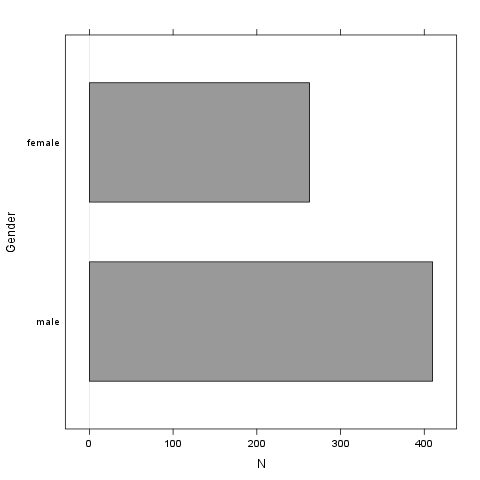
\includegraphics{3ed92ab3ffc6e875335e7e8c774c35a8.png}
\caption{}
\end{figure}

It seems that the highest value is \emph{2} which is exactly 2 times
higher than the smallest value (\emph{1}).

\subsection{\emph{age} (``Age'')}

The dataset has \emph{709} observations with \emph{677} valid values
(missing: \emph{32}) in \emph{age} (``Age''). This variable seems to be
numeric.

\subsubsection{Base statistics}

\ctable[pos = H, center, botcap]{llll}
{% notes
}
{% rows
\FL
\textbf{value} & \textbf{mean(age)} & \textbf{sd(age)} & \textbf{var(age)}
\ML
(all) & 24.5731 & 6.8491 & 46.9107
\LL
}

\subsubsection{Histogram}

\begin{figure}[htbp]
\centering
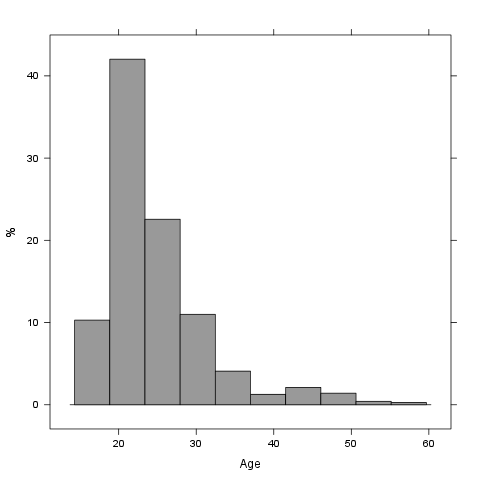
\includegraphics{ac5d789145bdef09b10219ef16429f53.png}
\caption{}
\end{figure}

It seems that the highest value is \emph{58} which is exactly 3.625
times higher than the smallest value (\emph{16}).

The standard deviation is 6.8491 (variance: 46.9107). The expected value
is around 24.5731, somewhere between 24.0572 and 25.0891 (SE: 0.2632).

If we suppose that \emph{Age} is not near to a normal distribution
(test: see below, skewness: 1.9296, kurtosis: 7.4851), checking the
median (23) might be a better option instead of the mean. The
interquartile range (6) measures the statistics dispersion of the
variable (similar to standard deviation) based on median.

\subsubsection{Normality tests}

\subsection{Introduction}

In statistics, \emph{normality} refers to an assumption that the
distribution of a random variable follows \emph{normal}
(\emph{Gaussian}) distribution. Because of its bell-like shape, it's
also known as the \emph{``bell curve''}. The formula for \emph{normal
distribution} is:

\[f(x) = \frac{1}{\sqrt{2\pi{}\sigma{}^2}} e^{-\frac{(x-\mu{})^2}{2\sigma{}^2}}\]

\emph{Normal distribution} belongs to a \emph{location-scale family} of
distributions, as it's defined two parameters:

\begin{itemize}
\item
  \emph{μ} - \emph{mean} or \emph{expectation} (location parameter)
\item
  \emph{σ\textsuperscript{2}} - \emph{variance} (scale parameter)
\end{itemize}
\begin{figure}[htbp]
\centering
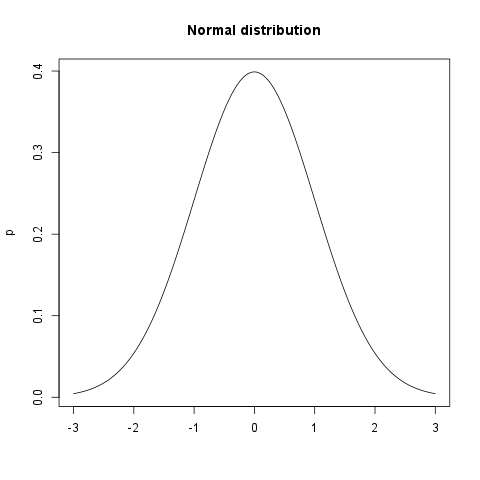
\includegraphics{2f8c434e103f36ec70966b372838d448.png}
\caption{}
\end{figure}

\subsection{Normality Tests}

\subsubsection{Overview}

Various hypothesis tests can be applied in order to test if the
distribution of given random variable violates normality assumption.
These procedures test the H\textsubscr{0} that provided variable's
distribution is \emph{normal}. At this point only few such tests will be
covered: the ones that are available in \texttt{stats} package (which
comes bundled with default R installation) and \texttt{nortest} package
that is
\href{http://cran.r-project.org/web/packages/nortest/index.html}{available}
on CRAN.

\begin{itemize}
\item
  \textbf{Shapiro-Wilk test} is a powerful normality test appropriate
  for small samples. In R, it's implemented in \texttt{shapiro.test}
  function available in \texttt{stats} package.
\item
  \textbf{Lilliefors test} is a modification of \emph{Kolmogorov-Smirnov
  test} appropriate for testing normality when parameters or normal
  distribution (\emph{μ}, \emph{σ\textsuperscript{2}}) are not known.
  \texttt{lillie.test} function is located in \texttt{nortest} package.
\item
  \textbf{Anderson-Darling test} is one of the most powerful normality
  tests as it will detect the most of departures from normality. You can
  find \texttt{ad.test} function in \texttt{nortest} package.
\item
  \textbf{Pearson Χ\textsuperscript{2} test} is another normality test
  which takes more ``traditional'' approach in normality testing.
  \texttt{pearson.test} is located in \texttt{nortest} package.
\end{itemize}
\subsubsection{Results}

Here you can see the results of applied normality tests (\emph{p-values}
less than 0.05 indicate significant discrepancies):

\ctable[pos = H, center, botcap]{lll}
{% notes
}
{% rows
\FL
 & \textbf{H} & \textbf{p}
\ML
shapiro.test & 0.8216 & 0
\\\noalign{\medskip}
lillie.test & 0.17 & 0
\\\noalign{\medskip}
ad.test & 32.1645 & 0
\\\noalign{\medskip}
pearson.test & 625.8479 & 0
\LL
}

So, let's draw some conclusions based on applied normality test:

\begin{itemize}
\item
  according to \emph{Shapiro-Wilk test}, the distribution of \emph{Age}
  is not normal.
\item
  based on \emph{Lilliefors test}, distribution of \emph{Age} is not
  normal
\item
  \emph{Anderson-Darling test} confirms violation of normality
  assumption
\item
  \emph{Pearson's Χ\textsuperscript{2} test} classifies the underlying
  distribution as non-normal
\end{itemize}
\subsection{Diagnostic Plots}

There are various plots that can help you decide about the normality of
the distribution. Only a few most commonly used plots will be shown:
\emph{histogram}, \emph{Q-Q plot} and \emph{kernel density plot}.

\subsubsection{Histogram}

\emph{Histogram} was first introduced by \emph{Karl Pearson} and it's
probably the most popular plot for depicting the probability
distribution of a random variable. However, the decision depends on
number of bins, so it can sometimes be misleading. If the variable
distribution is normal, bins should resemble the ``bell-like'' shape.

\begin{figure}[htbp]
\centering
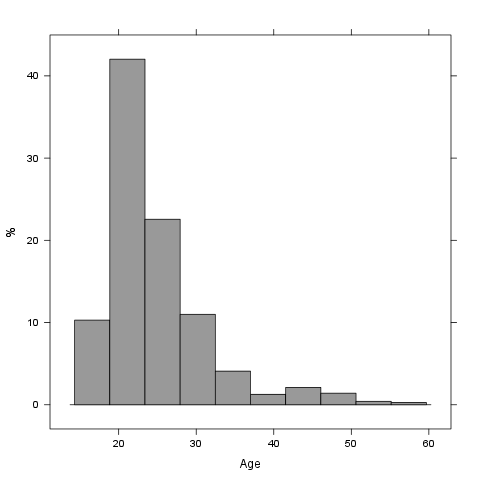
\includegraphics{ac5d789145bdef09b10219ef16429f53.png}
\caption{}
\end{figure}

\subsubsection{Q-Q Plot}

``Q'' in \emph{Q-Q plot} stands for \emph{quantile}, as this plot
compares empirical and theoretical distribution (in this case,
\emph{normal} distribution) by plotting their quantiles against each
other. For normal distribution, plotted dots should approximate a
``straight'', \texttt{x = y} line.

\begin{figure}[htbp]
\centering
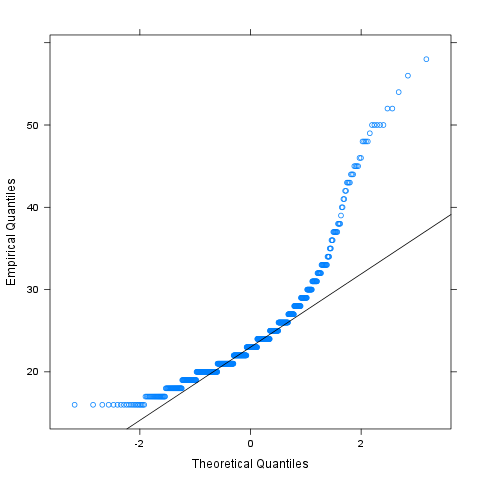
\includegraphics{cbbba756d844aa053998959b73b9feff.png}
\caption{}
\end{figure}

\subsubsection{Kernel Density Plot}

\emph{Kernel density plot} is a plot of smoothed \emph{empirical
distribution function}. As such, it provides good insight about the
shape of the distribution. For normal distributions, it should resemble
the well known ``bell shape''.

\begin{figure}[htbp]
\centering
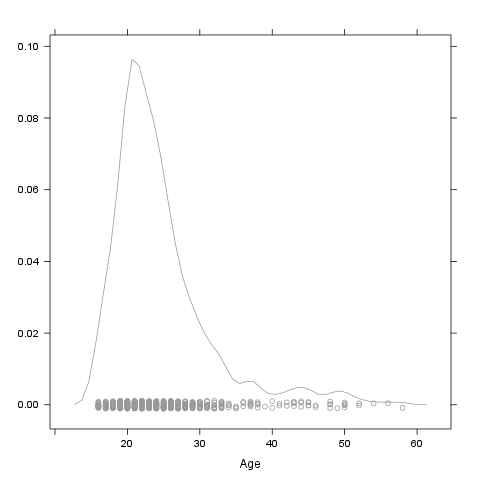
\includegraphics{6fd0494eea748495baa80653752f194f.png}
\caption{}
\end{figure}

\subsection{Description}

This template will return descriptive statistics of numerical or
frequency tables of categorical variables.

\subsection{\emph{chatim} (``Chat \& IM usage'')}

The dataset has \emph{709} observations with \emph{669} valid values
(missing: \emph{40}) in \emph{chatim} (``Chat \& IM usage''). This
variable seems to be a factor.

\subsubsection{Base statistics}

\ctable[pos = H, center, botcap]{llllll}
{% notes
}
{% rows
\FL
 & \textbf{chatim} & \textbf{N} & \textbf{pct} & \textbf{cumul.count} & \textbf{cumul.pct}
\ML
1 & never & 60 & 8.9686 & 60 & 8.9686
\\\noalign{\medskip}
2 & very rarely & 73 & 10.9118 & 133 & 19.8804
\\\noalign{\medskip}
3 & rarely & 58 & 8.6697 & 191 & 28.5501
\\\noalign{\medskip}
4 & sometimes & 113 & 16.8909 & 304 & 45.441
\\\noalign{\medskip}
5 & often & 136 & 20.3288 & 440 & 65.7698
\\\noalign{\medskip}
6 & very often & 88 & 13.154 & 528 & 78.9238
\\\noalign{\medskip}
7 & always & 141 & 21.0762 & 669 & 100
\\\noalign{\medskip}
Total &  & 669 & 100 & 669 & 100
\LL
}

\subsubsection{Barplot}

\begin{figure}[htbp]
\centering
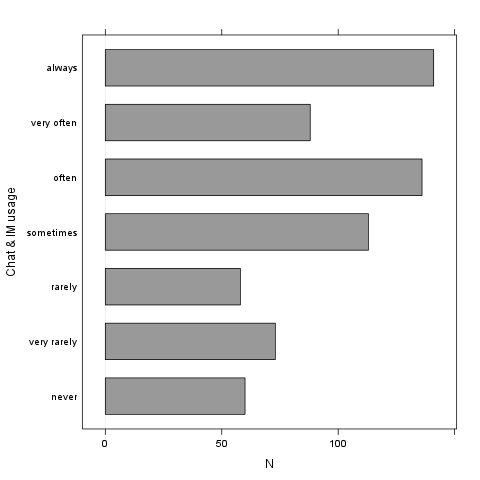
\includegraphics{5a00abbe4c793ceedbbf10939665b5cf.png}
\caption{}
\end{figure}

It seems that the highest value is \emph{7} which is exactly 7 times
higher than the smallest value (\emph{1}).

\subsection{\emph{game} (``On-line games usage'')}

The dataset has \emph{709} observations with \emph{677} valid values
(missing: \emph{32}) in \emph{game} (``On-line games usage''). This
variable seems to be a factor.

\subsubsection{Base statistics}

\ctable[pos = H, center, botcap]{llllll}
{% notes
}
{% rows
\FL
 & \textbf{game} & \textbf{N} & \textbf{pct} & \textbf{cumul.count} & \textbf{cumul.pct}
\ML
1 & never & 352 & 51.9941 & 352 & 51.9941
\\\noalign{\medskip}
2 & very rarely & 128 & 18.9069 & 480 & 70.901
\\\noalign{\medskip}
3 & rarely & 32 & 4.7267 & 512 & 75.6278
\\\noalign{\medskip}
4 & sometimes & 60 & 8.8626 & 572 & 84.4904
\\\noalign{\medskip}
5 & often & 37 & 5.4653 & 609 & 89.9557
\\\noalign{\medskip}
6 & very often & 35 & 5.1699 & 644 & 95.1256
\\\noalign{\medskip}
7 & always & 33 & 4.8744 & 677 & 100
\\\noalign{\medskip}
Total &  & 677 & 100 & 677 & 100
\LL
}

\subsubsection{Barplot}

\begin{figure}[htbp]
\centering
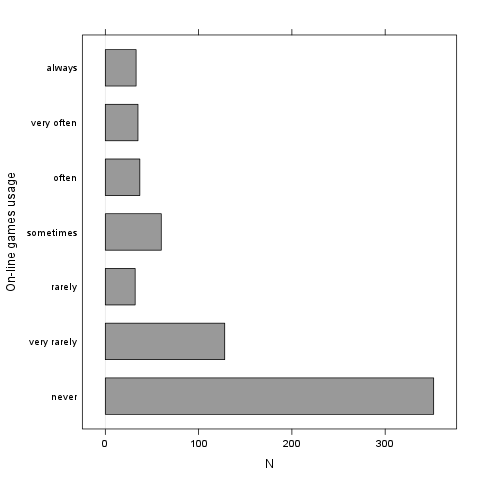
\includegraphics{e53046a09491443064e085131e547971.png}
\caption{}
\end{figure}

It seems that the highest value is \emph{7} which is exactly 7 times
higher than the smallest value (\emph{1}).

\subsection{\emph{surf} (``Web surfing usage'')}

The dataset has \emph{709} observations with \emph{678} valid values
(missing: \emph{31}) in \emph{surf} (``Web surfing usage''). This
variable seems to be a factor.

\subsubsection{Base statistics}

\ctable[pos = H, center, botcap]{llllll}
{% notes
}
{% rows
\FL
 & \textbf{surf} & \textbf{N} & \textbf{pct} & \textbf{cumul.count} & \textbf{cumul.pct}
\ML
1 & never & 17 & 2.5074 & 17 & 2.5074
\\\noalign{\medskip}
2 & very rarely & 26 & 3.8348 & 43 & 6.3422
\\\noalign{\medskip}
3 & rarely & 33 & 4.8673 & 76 & 11.2094
\\\noalign{\medskip}
4 & sometimes & 107 & 15.7817 & 183 & 26.9912
\\\noalign{\medskip}
5 & often & 158 & 23.3038 & 341 & 50.295
\\\noalign{\medskip}
6 & very often & 142 & 20.944 & 483 & 71.2389
\\\noalign{\medskip}
7 & always & 195 & 28.7611 & 678 & 100
\\\noalign{\medskip}
Total &  & 678 & 100 & 678 & 100
\LL
}

\subsubsection{Barplot}

\begin{figure}[htbp]
\centering
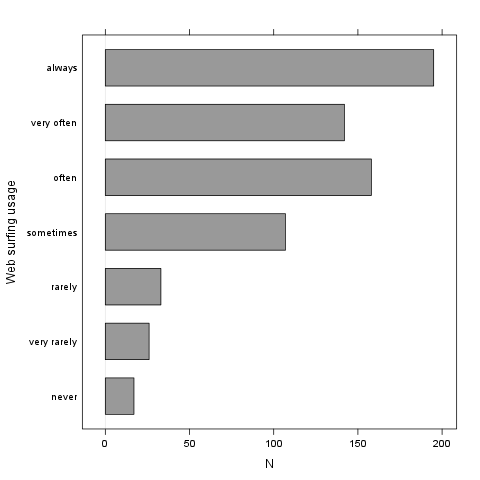
\includegraphics{0166a8b5df2f3db871e8736bfee8af6e.png}
\caption{}
\end{figure}

It seems that the highest value is \emph{7} which is exactly 7 times
higher than the smallest value (\emph{1}).

\subsection{\emph{email} (``Email usage'')}

The dataset has \emph{709} observations with \emph{672} valid values
(missing: \emph{37}) in \emph{email} (``Email usage''). This variable
seems to be a factor.

\subsubsection{Base statistics}

\ctable[pos = H, center, botcap]{llllll}
{% notes
}
{% rows
\FL
 & \textbf{email} & \textbf{N} & \textbf{pct} & \textbf{cumul.count} & \textbf{cumul.pct}
\ML
1 & never & 13 & 1.9345 & 13 & 1.9345
\\\noalign{\medskip}
2 & very rarely & 36 & 5.3571 & 49 & 7.2917
\\\noalign{\medskip}
3 & rarely & 46 & 6.8452 & 95 & 14.1369
\\\noalign{\medskip}
4 & sometimes & 87 & 12.9464 & 182 & 27.0833
\\\noalign{\medskip}
5 & often & 123 & 18.3036 & 305 & 45.3869
\\\noalign{\medskip}
6 & very often & 108 & 16.0714 & 413 & 61.4583
\\\noalign{\medskip}
7 & always & 259 & 38.5417 & 672 & 100
\\\noalign{\medskip}
Total &  & 672 & 100 & 672 & 100
\LL
}

\subsubsection{Barplot}

\begin{figure}[htbp]
\centering
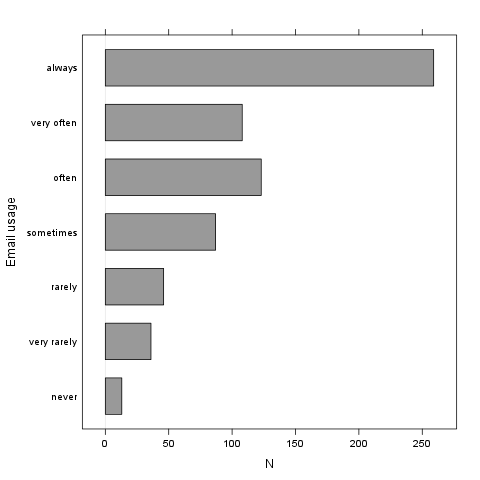
\includegraphics{895cde198b269bf65b01e1e067a515c8.png}
\caption{}
\end{figure}

It seems that the highest value is \emph{7} which is exactly 7 times
higher than the smallest value (\emph{1}).

\subsection{\emph{download} (``Download usage'')}

The dataset has \emph{709} observations with \emph{677} valid values
(missing: \emph{32}) in \emph{download} (``Download usage''). This
variable seems to be a factor.

\subsubsection{Base statistics}

\ctable[pos = H, center, botcap]{llllll}
{% notes
}
{% rows
\FL
 & \textbf{download} & \textbf{N} & \textbf{pct} & \textbf{cumul.count} & \textbf{cumul.pct}
\ML
1 & never & 11 & 1.6248 & 11 & 1.6248
\\\noalign{\medskip}
2 & very rarely & 28 & 4.1359 & 39 & 5.7607
\\\noalign{\medskip}
3 & rarely & 29 & 4.2836 & 68 & 10.0443
\\\noalign{\medskip}
4 & sometimes & 80 & 11.8168 & 148 & 21.8612
\\\noalign{\medskip}
5 & often & 124 & 18.3161 & 272 & 40.1773
\\\noalign{\medskip}
6 & very often & 160 & 23.6337 & 432 & 63.8109
\\\noalign{\medskip}
7 & always & 245 & 36.1891 & 677 & 100
\\\noalign{\medskip}
Total &  & 677 & 100 & 677 & 100
\LL
}

\subsubsection{Barplot}

\begin{figure}[htbp]
\centering
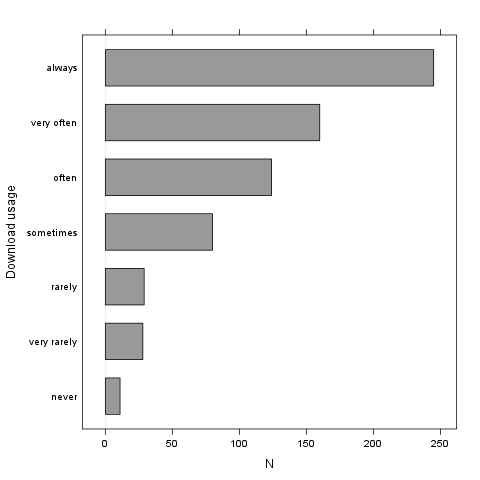
\includegraphics{dde181184885b8777d0248b3f421289a.png}
\caption{}
\end{figure}

It seems that the highest value is \emph{7} which is exactly 7 times
higher than the smallest value (\emph{1}).

\subsection{\emph{forum} (``Web forums usage'')}

The dataset has \emph{709} observations with \emph{673} valid values
(missing: \emph{36}) in \emph{forum} (``Web forums usage''). This
variable seems to be a factor.

\subsubsection{Base statistics}

\ctable[pos = H, center, botcap]{llllll}
{% notes
}
{% rows
\FL
 & \textbf{forum} & \textbf{N} & \textbf{pct} & \textbf{cumul.count} & \textbf{cumul.pct}
\ML
1 & never & 76 & 11.2927 & 76 & 11.2927
\\\noalign{\medskip}
2 & very rarely & 80 & 11.8871 & 156 & 23.1798
\\\noalign{\medskip}
3 & rarely & 72 & 10.6984 & 228 & 33.8782
\\\noalign{\medskip}
4 & sometimes & 111 & 16.4933 & 339 & 50.3715
\\\noalign{\medskip}
5 & often & 109 & 16.1961 & 448 & 66.5676
\\\noalign{\medskip}
6 & very often & 119 & 17.682 & 567 & 84.2496
\\\noalign{\medskip}
7 & always & 106 & 15.7504 & 673 & 100
\\\noalign{\medskip}
Total &  & 673 & 100 & 673 & 100
\LL
}

\subsubsection{Barplot}

\begin{figure}[htbp]
\centering
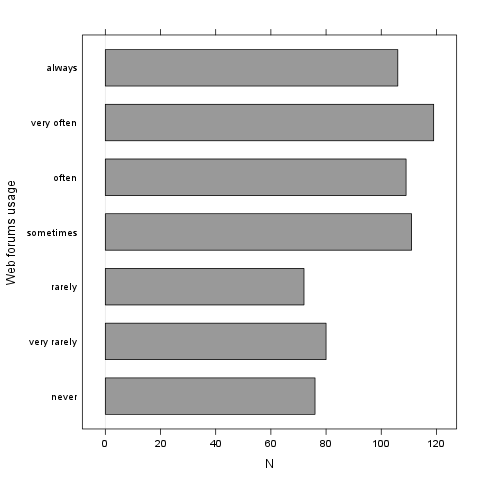
\includegraphics{ac419134b2f4695e544d8886ba12e0c2.png}
\caption{}
\end{figure}

It seems that the highest value is \emph{7} which is exactly 7 times
higher than the smallest value (\emph{1}).

\subsection{\emph{socnet} (``Social networks usage'')}

The dataset has \emph{709} observations with \emph{678} valid values
(missing: \emph{31}) in \emph{socnet} (``Social networks usage''). This
variable seems to be a factor.

\subsubsection{Base statistics}

\ctable[pos = H, center, botcap]{llllll}
{% notes
}
{% rows
\FL
 & \textbf{socnet} & \textbf{N} & \textbf{pct} & \textbf{cumul.count} & \textbf{cumul.pct}
\ML
1 & never & 208 & 30.6785 & 208 & 30.6785
\\\noalign{\medskip}
2 & very rarely & 102 & 15.0442 & 310 & 45.7227
\\\noalign{\medskip}
3 & rarely & 57 & 8.4071 & 367 & 54.1298
\\\noalign{\medskip}
4 & sometimes & 87 & 12.8319 & 454 & 66.9617
\\\noalign{\medskip}
5 & often & 79 & 11.6519 & 533 & 78.6136
\\\noalign{\medskip}
6 & very often & 80 & 11.7994 & 613 & 90.413
\\\noalign{\medskip}
7 & always & 65 & 9.587 & 678 & 100
\\\noalign{\medskip}
Total &  & 678 & 100 & 678 & 100
\LL
}

\subsubsection{Barplot}

\begin{figure}[htbp]
\centering
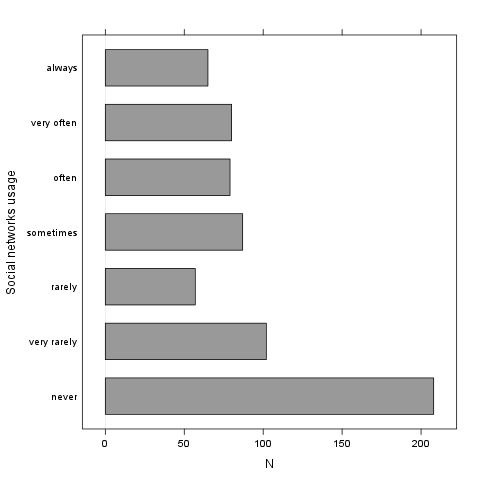
\includegraphics{8475d98870c1cdd2436a3abdb0d69a66.png}
\caption{}
\end{figure}

It seems that the highest value is \emph{7} which is exactly 7 times
higher than the smallest value (\emph{1}).

\subsection{\emph{xxx} (``Adult sites usage'')}

The dataset has \emph{709} observations with \emph{674} valid values
(missing: \emph{35}) in \emph{xxx} (``Adult sites usage''). This
variable seems to be a factor.

\subsubsection{Base statistics}

\ctable[pos = H, center, botcap]{llllll}
{% notes
}
{% rows
\FL
 & \textbf{xxx} & \textbf{N} & \textbf{pct} & \textbf{cumul.count} & \textbf{cumul.pct}
\ML
1 & never & 274 & 40.6528 & 274 & 40.6528
\\\noalign{\medskip}
2 & very rarely & 124 & 18.3976 & 398 & 59.0504
\\\noalign{\medskip}
3 & rarely & 52 & 7.7151 & 450 & 66.7656
\\\noalign{\medskip}
4 & sometimes & 131 & 19.4362 & 581 & 86.2018
\\\noalign{\medskip}
5 & often & 46 & 6.8249 & 627 & 93.0267
\\\noalign{\medskip}
6 & very often & 28 & 4.1543 & 655 & 97.181
\\\noalign{\medskip}
7 & always & 19 & 2.819 & 674 & 100
\\\noalign{\medskip}
Total &  & 674 & 100 & 674 & 100
\LL
}

\subsubsection{Barplot}

\begin{figure}[htbp]
\centering
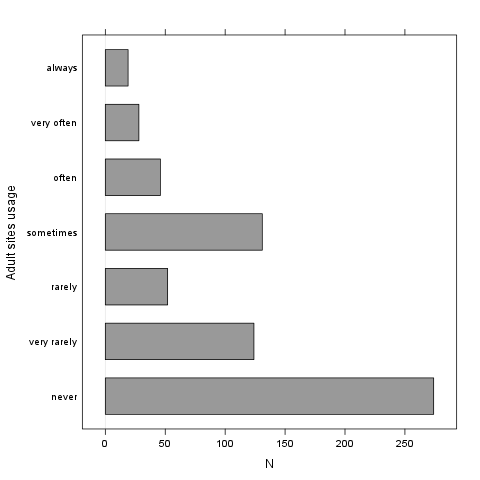
\includegraphics{4fda8cf992e8de93624c45ef3c72a0c5.png}
\caption{}
\end{figure}

It seems that the highest value is \emph{7} which is exactly 7 times
higher than the smallest value (\emph{1}).

\subsection{Description}

This template will return descriptive statistics of numerical or
frequency tables of categorical variables.

\subsection{\emph{hp}}

The dataset has \emph{32} observations with \emph{32} valid values
(missing: \emph{0}) in \emph{hp}. This variable seems to be numeric.

\subsubsection{Base statistics}

\ctable[pos = H, center, botcap]{llll}
{% notes
}
{% rows
\FL
\textbf{value} & \textbf{mean(hp)} & \textbf{sd(hp)} & \textbf{var(hp)}
\ML
(all) & 146.6875 & 68.5629 & 4700.8669
\LL
}

\subsubsection{Histogram}

\begin{figure}[htbp]
\centering
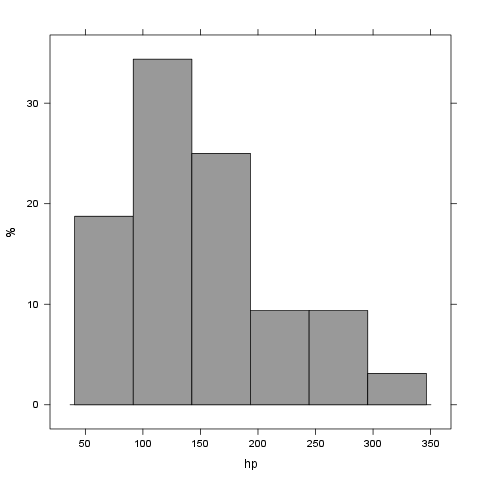
\includegraphics{d90ec4a0af55fabeae7988710a062ce0.png}
\caption{}
\end{figure}

It seems that the highest value is \emph{335} which is exactly 6.4423
times higher than the smallest value (\emph{52}).

The standard deviation is 68.5629 (variance: 4700.8669). The expected
value is around 146.6875, somewhere between 122.9317 and 170.4433 (SE:
12.1203).

If we suppose that \emph{hp} is not near to a normal distribution (test:
see below, skewness: 0.7614, kurtosis: 3.0522), checking the median
(123) might be a better option instead of the mean. The interquartile
range (83.5) measures the statistics dispersion of the variable (similar
to standard deviation) based on median.

\subsubsection{Normality tests}

\subsection{Introduction}

In statistics, \emph{normality} refers to an assumption that the
distribution of a random variable follows \emph{normal}
(\emph{Gaussian}) distribution. Because of its bell-like shape, it's
also known as the \emph{``bell curve''}. The formula for \emph{normal
distribution} is:

\[f(x) = \frac{1}{\sqrt{2\pi{}\sigma{}^2}} e^{-\frac{(x-\mu{})^2}{2\sigma{}^2}}\]

\emph{Normal distribution} belongs to a \emph{location-scale family} of
distributions, as it's defined two parameters:

\begin{itemize}
\item
  \emph{μ} - \emph{mean} or \emph{expectation} (location parameter)
\item
  \emph{σ\textsuperscript{2}} - \emph{variance} (scale parameter)
\end{itemize}
\begin{figure}[htbp]
\centering
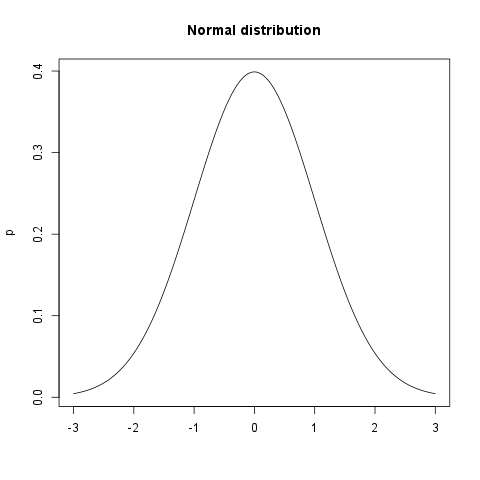
\includegraphics{2f8c434e103f36ec70966b372838d448.png}
\caption{}
\end{figure}

\subsection{Normality Tests}

\subsubsection{Overview}

Various hypothesis tests can be applied in order to test if the
distribution of given random variable violates normality assumption.
These procedures test the H\textsubscr{0} that provided variable's
distribution is \emph{normal}. At this point only few such tests will be
covered: the ones that are available in \texttt{stats} package (which
comes bundled with default R installation) and \texttt{nortest} package
that is
\href{http://cran.r-project.org/web/packages/nortest/index.html}{available}
on CRAN.

\begin{itemize}
\item
  \textbf{Shapiro-Wilk test} is a powerful normality test appropriate
  for small samples. In R, it's implemented in \texttt{shapiro.test}
  function available in \texttt{stats} package.
\item
  \textbf{Lilliefors test} is a modification of \emph{Kolmogorov-Smirnov
  test} appropriate for testing normality when parameters or normal
  distribution (\emph{μ}, \emph{σ\textsuperscript{2}}) are not known.
  \texttt{lillie.test} function is located in \texttt{nortest} package.
\item
  \textbf{Anderson-Darling test} is one of the most powerful normality
  tests as it will detect the most of departures from normality. You can
  find \texttt{ad.test} function in \texttt{nortest} package.
\item
  \textbf{Pearson Χ\textsuperscript{2} test} is another normality test
  which takes more ``traditional'' approach in normality testing.
  \texttt{pearson.test} is located in \texttt{nortest} package.
\end{itemize}
\subsubsection{Results}

Here you can see the results of applied normality tests (\emph{p-values}
less than 0.05 indicate significant discrepancies):

\ctable[pos = H, center, botcap]{lll}
{% notes
}
{% rows
\FL
 & \textbf{H} & \textbf{p}
\ML
shapiro.test & 0.9334 & 0.0488
\\\noalign{\medskip}
lillie.test & 0.1664 & 0.0245
\\\noalign{\medskip}
ad.test & 0.7077 & 0.0584
\\\noalign{\medskip}
pearson.test & 11.5 & 0.0423
\LL
}

So, let's draw some conclusions based on applied normality test:

\begin{itemize}
\item
  according to \emph{Shapiro-Wilk test}, the distribution of \emph{hp}
  is not normal.
\item
  based on \emph{Lilliefors test}, distribution of \emph{hp} is not
  normal
\item
  \emph{Anderson-Darling test} confirms normality assumption
\item
  \emph{Pearson's Χ\textsuperscript{2} test} classifies the underlying
  distribution as non-normal
\end{itemize}
\subsection{Diagnostic Plots}

There are various plots that can help you decide about the normality of
the distribution. Only a few most commonly used plots will be shown:
\emph{histogram}, \emph{Q-Q plot} and \emph{kernel density plot}.

\subsubsection{Histogram}

\emph{Histogram} was first introduced by \emph{Karl Pearson} and it's
probably the most popular plot for depicting the probability
distribution of a random variable. However, the decision depends on
number of bins, so it can sometimes be misleading. If the variable
distribution is normal, bins should resemble the ``bell-like'' shape.

\begin{figure}[htbp]
\centering
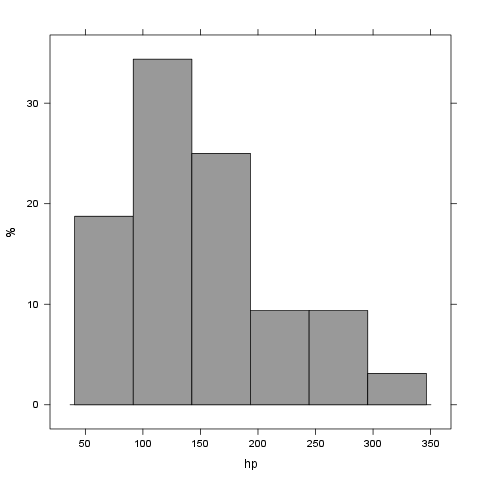
\includegraphics{d90ec4a0af55fabeae7988710a062ce0.png}
\caption{}
\end{figure}

\subsubsection{Q-Q Plot}

``Q'' in \emph{Q-Q plot} stands for \emph{quantile}, as this plot
compares empirical and theoretical distribution (in this case,
\emph{normal} distribution) by plotting their quantiles against each
other. For normal distribution, plotted dots should approximate a
``straight'', \texttt{x = y} line.

\begin{figure}[htbp]
\centering
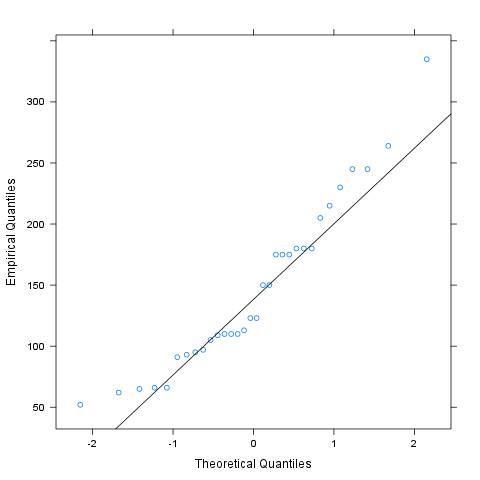
\includegraphics{17e5c77b83c6e3e636487406decc14c7.png}
\caption{}
\end{figure}

\subsubsection{Kernel Density Plot}

\emph{Kernel density plot} is a plot of smoothed \emph{empirical
distribution function}. As such, it provides good insight about the
shape of the distribution. For normal distributions, it should resemble
the well known ``bell shape''.

\begin{figure}[htbp]
\centering
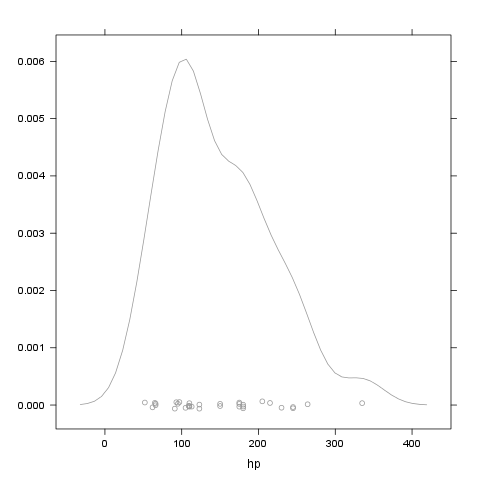
\includegraphics{135de2b4d3cb1b1a3ece741c584c0a59.png}
\caption{}
\end{figure}

\subsection{\emph{wt}}

The dataset has \emph{32} observations with \emph{32} valid values
(missing: \emph{0}) in \emph{wt}. This variable seems to be numeric.

\subsubsection{Base statistics}

\ctable[pos = H, center, botcap]{llll}
{% notes
}
{% rows
\FL
\textbf{value} & \textbf{mean(wt)} & \textbf{sd(wt)} & \textbf{var(wt)}
\ML
(all) & 3.2172 & 0.9785 & 0.9574
\LL
}

\subsubsection{Histogram}

\begin{figure}[htbp]
\centering
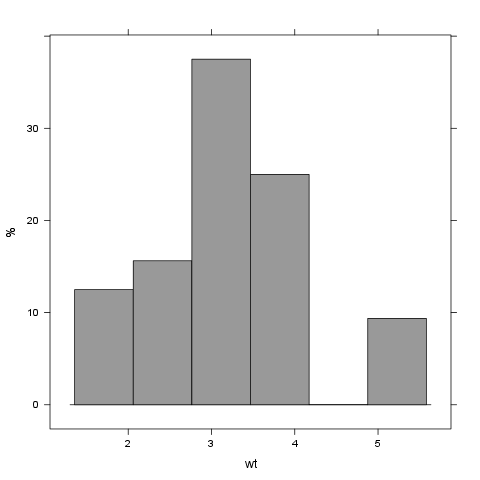
\includegraphics{10caa8222b28328a6d8fd28917cbfb45.png}
\caption{}
\end{figure}

It seems that the highest value is \emph{5.424} which is exactly 3.5849
times higher than the smallest value (\emph{1.513}).

The standard deviation is 0.9785 (variance: 0.9574). The expected value
is around 3.2172, somewhere between 2.8782 and 3.5563 (SE: 0.173).

If we suppose that \emph{wt} is not near to a normal distribution (test:
see below, skewness: 0.4438, kurtosis: 3.1725), checking the median
(3.325) might be a better option instead of the mean. The interquartile
range (1.0288) measures the statistics dispersion of the variable
(similar to standard deviation) based on median.

\subsubsection{Normality tests}

\subsection{Introduction}

In statistics, \emph{normality} refers to an assumption that the
distribution of a random variable follows \emph{normal}
(\emph{Gaussian}) distribution. Because of its bell-like shape, it's
also known as the \emph{``bell curve''}. The formula for \emph{normal
distribution} is:

\[f(x) = \frac{1}{\sqrt{2\pi{}\sigma{}^2}} e^{-\frac{(x-\mu{})^2}{2\sigma{}^2}}\]

\emph{Normal distribution} belongs to a \emph{location-scale family} of
distributions, as it's defined two parameters:

\begin{itemize}
\item
  \emph{μ} - \emph{mean} or \emph{expectation} (location parameter)
\item
  \emph{σ\textsuperscript{2}} - \emph{variance} (scale parameter)
\end{itemize}
\begin{figure}[htbp]
\centering
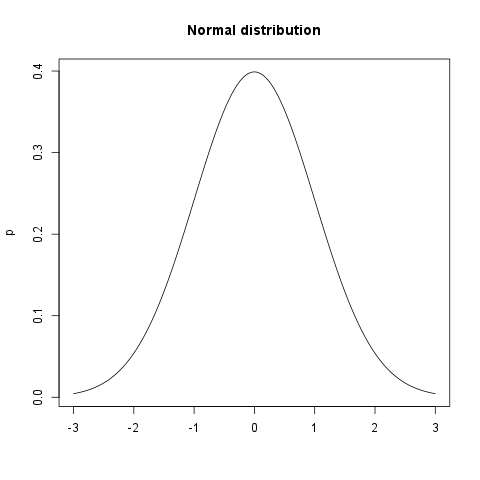
\includegraphics{2f8c434e103f36ec70966b372838d448.png}
\caption{}
\end{figure}

\subsection{Normality Tests}

\subsubsection{Overview}

Various hypothesis tests can be applied in order to test if the
distribution of given random variable violates normality assumption.
These procedures test the H\textsubscr{0} that provided variable's
distribution is \emph{normal}. At this point only few such tests will be
covered: the ones that are available in \texttt{stats} package (which
comes bundled with default R installation) and \texttt{nortest} package
that is
\href{http://cran.r-project.org/web/packages/nortest/index.html}{available}
on CRAN.

\begin{itemize}
\item
  \textbf{Shapiro-Wilk test} is a powerful normality test appropriate
  for small samples. In R, it's implemented in \texttt{shapiro.test}
  function available in \texttt{stats} package.
\item
  \textbf{Lilliefors test} is a modification of \emph{Kolmogorov-Smirnov
  test} appropriate for testing normality when parameters or normal
  distribution (\emph{μ}, \emph{σ\textsuperscript{2}}) are not known.
  \texttt{lillie.test} function is located in \texttt{nortest} package.
\item
  \textbf{Anderson-Darling test} is one of the most powerful normality
  tests as it will detect the most of departures from normality. You can
  find \texttt{ad.test} function in \texttt{nortest} package.
\item
  \textbf{Pearson Χ\textsuperscript{2} test} is another normality test
  which takes more ``traditional'' approach in normality testing.
  \texttt{pearson.test} is located in \texttt{nortest} package.
\end{itemize}
\subsubsection{Results}

Here you can see the results of applied normality tests (\emph{p-values}
less than 0.05 indicate significant discrepancies):

\ctable[pos = H, center, botcap]{lll}
{% notes
}
{% rows
\FL
 & \textbf{H} & \textbf{p}
\ML
shapiro.test & 0.9433 & 0.0927
\\\noalign{\medskip}
lillie.test & 0.1356 & 0.1412
\\\noalign{\medskip}
ad.test & 0.6091 & 0.1038
\\\noalign{\medskip}
pearson.test & 4.5 & 0.4799
\LL
}

So, let's draw some conclusions based on applied normality test:

\begin{itemize}
\item
  according to \emph{Shapiro-Wilk test}, the distribution of \emph{wt}
  is normal.
\item
  based on \emph{Lilliefors test}, distribution of \emph{wt} is not
  normal
\item
  \emph{Anderson-Darling test} confirms normality assumption
\item
  \emph{Pearson's Χ\textsuperscript{2} test} classifies the underlying
  distribution as non-normal
\end{itemize}
\subsection{Diagnostic Plots}

There are various plots that can help you decide about the normality of
the distribution. Only a few most commonly used plots will be shown:
\emph{histogram}, \emph{Q-Q plot} and \emph{kernel density plot}.

\subsubsection{Histogram}

\emph{Histogram} was first introduced by \emph{Karl Pearson} and it's
probably the most popular plot for depicting the probability
distribution of a random variable. However, the decision depends on
number of bins, so it can sometimes be misleading. If the variable
distribution is normal, bins should resemble the ``bell-like'' shape.

\begin{figure}[htbp]
\centering
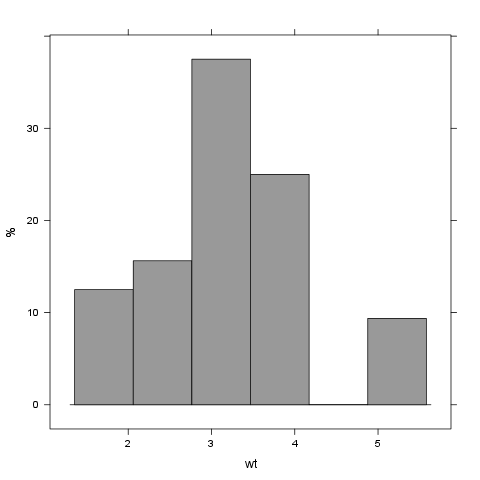
\includegraphics{10caa8222b28328a6d8fd28917cbfb45.png}
\caption{}
\end{figure}

\subsubsection{Q-Q Plot}

``Q'' in \emph{Q-Q plot} stands for \emph{quantile}, as this plot
compares empirical and theoretical distribution (in this case,
\emph{normal} distribution) by plotting their quantiles against each
other. For normal distribution, plotted dots should approximate a
``straight'', \texttt{x = y} line.

\begin{figure}[htbp]
\centering
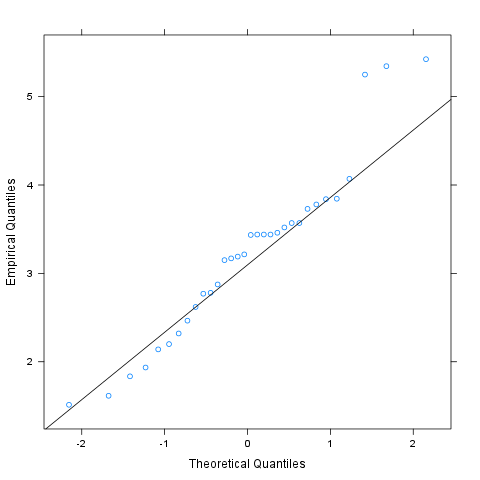
\includegraphics{ff471a5bcb80aaf91b4c053ab038d69a.png}
\caption{}
\end{figure}

\subsubsection{Kernel Density Plot}

\emph{Kernel density plot} is a plot of smoothed \emph{empirical
distribution function}. As such, it provides good insight about the
shape of the distribution. For normal distributions, it should resemble
the well known ``bell shape''.

\begin{figure}[htbp]
\centering
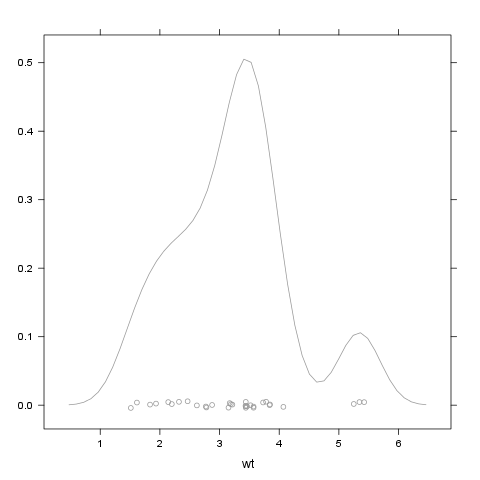
\includegraphics{16a7d5cf96ceceffd6db59f9a2514dce.png}
\caption{}
\end{figure}

\begin{center}\rule{3in}{0.4pt}\end{center}

This report was generated with
\href{http://rapport-package.info/}{rapport}.

\begin{figure}[htbp]
\centering

\includegraphics{images/rapport.png}
\caption{}
\end{figure}

\end{document}
